\documentclass[conference]{IEEEtran}
% IEEE WCNC 2027 -- 6-page hard limit (10pt), single-blind (author names shown).
% This is the NON-STATIONARY / joint TWT+OFDMA study. It is a separate paper from
% the earlier submission in wcnc2027-paper/, which is left untouched.

\usepackage{cite}
\usepackage{amsmath,amssymb,amsfonts}
\usepackage{algorithm}
\usepackage{algorithmic}
\usepackage{graphicx}
\usepackage{textcomp}
\usepackage{xcolor}
\usepackage{booktabs}
\usepackage{multirow}
\usepackage{url}

\renewcommand{\topfraction}{0.92}
\renewcommand{\bottomfraction}{0.85}
\renewcommand{\textfraction}{0.08}
\renewcommand{\floatpagefraction}{0.75}
\setcounter{topnumber}{3}
\setcounter{totalnumber}{4}

\def\BibTeX{{\rm B\kern-.05em{\sc i\kern-.025em b}\kern-.08em
    T\kern-.1667em\lower.7ex\hbox{E}\kern-.125emX}}

\begin{document}

\title{Do Target Wake Time and Uplink OFDMA Combine?\\
An Offline Reinforcement Learning Study of Joint\\
Scheduling in IEEE 802.11ax}

\author{
\IEEEauthorblockN{Ahmed Selim Anwar, Ahmed Maksud, Joarder Jafor Sadique,\\
Charles Wiame, and Marcelo Menezes De Carvalho}
\IEEEauthorblockA{\textit{Department of Electrical Engineering}, \textit{Texas State University},
San Marcos, TX, USA\\
Emails: \{ahmed.selim.anwar, poy18, jjsadique, cwiame, mmcarvalho\}@txstate.edu}
}

\maketitle
\begin{abstract}
IEEE 802.11ax introduces Target Wake Time (TWT) and uplink OFDMA to reduce
station energy in dense Wi-Fi deployments.
The two mechanisms are usually configured separately, and no study measures
station energy when an access point controls both.
The difficulty is that a controller must adapt to changing traffic, yet online
learning is impractical in a production network, and a hand-tuned rule needs an
expert and is unlikely to be optimal.
Offline reinforcement learning avoids both: a policy is trained from logged
data alone, with no exploration on the live network.
We cast joint control as a 760-way action, selecting a TWT schedule, a
station-to-group assignment, and whether uplink OFDMA is enabled at each
decision, and train five offline algorithms on 100{,}235 logged transitions in
ns-3.44.
Implicit Q-Learning reaches $107.3$\,J against a tuned hand-designed
controller's $166.5$\,J, a $35.6\,\%$ reduction at higher throughput, and does
so consistently: the spread over ten training runs is $2.6$\,J. Four of the
five methods lose to that controller, and the energy of all five is ordered by
how often each enables uplink OFDMA.
\end{abstract}

\begin{IEEEkeywords}
IEEE 802.11ax, Target Wake Time, uplink OFDMA, offline reinforcement learning,
energy efficiency, conservative Q-learning, off-policy evaluation.
\end{IEEEkeywords}
\section{Introduction}

IEEE 802.11ax gives an access point two ways to cut the energy cost of
battery-powered stations. Target Wake Time (TWT) schedules when each station
wakes, so radios sleep between service
periods~\cite{chen2019twt,qiu2021category}. Uplink OFDMA replaces contention
with scheduled resource units, so several stations transmit at
once~\cite{kotagiri2021distributed,han2024multiagent}. Both reduce energy, and
recent work treats their configuration as a scheduling problem of its
own~\cite{busacca2026twt,liu2025priority}.

The two mechanisms are normally configured in isolation. TWT studies fix the
OFDMA setting, and OFDMA studies fix or ignore the sleep
schedule~\cite{karaca2020joint,noh2024joint}. Yet they compete for the same
resource: a trigger frame is only useful to a station awake to receive it, so
every OFDMA round draws on the airtime and the radio states TWT is trying to
conserve.

No single setting serves a whole cell. A basic service set carries mixed
traffic---latency-sensitive video, periodic telemetry and voice
together~\cite{yang2021twt,tan2024drl}---and a schedule tuned for light
telemetry is wasteful under a video burst. A controller must adapt, which
raises how it should be obtained.

A hand-coded rule is cheap to run but needs an expert to tune, and is unlikely
to stay optimal away from the conditions it was tuned for. An idealised online
learner could in principle track the optimum instant by instant, but it must
explore on the live network, and exploration costs latency and risks service
degradation~\cite{wydmanski2021contention,yang2024offline}.

Offline reinforcement learning avoids both
costs~\cite{levine2020offline}. A policy is trained from an already-collected
dataset and never acts on the network while learning, so it needs neither
exploration nor expert-labelled actions---though the state features, reward and
action catalogue remain design choices. The price is
distribution shift, for which conservative value estimation is the standard
remedy~\cite{kumar2020cql,kostrikov2022iql}. Its wireless applications
concentrate on cellular resource
management~\cite{yang2024offline,eldeeb2026marl}, leaving Wi-Fi power save
largely unexamined.

We apply it to joint TWT and OFDMA control. Once per decision window the
access point selects a TWT schedule, a station-to-group assignment and whether
uplink OFDMA is enabled---a 760-way discrete action. Making the OFDMA bit part
of the action rather than a property of the run is what makes the problem
joint. Five offline algorithms are trained on $100{,}235$ transitions logged in
ns-3.44 and compared against hand-designed and non-adaptive baselines.

Our contributions are the following.\footnote{Code, the ns-3 scenario and the
frozen results that generate every table and figure:
\url{https://github.com/shuvo102459/802.11ax-OfflineRL-TWT-OFDMA}}
\begin{itemize}
\item A policy learned without online interaction or expert-set thresholds that
cuts station energy against a tuned hand-designed controller at higher
throughput, holding across ten training runs and against every fixed schedule
tested---its advantage coming from switching schedules, not from finding a
better static one.
\item Evidence that at this operating point enabling the uplink scheduler
raises energy at every TWT configuration tested, with five independently trained
policies ordering by energy as they order by how often each enables it.
\item A service-period-aligned trigger scheduler that solicits a station only
while its service period can contain the whole exchange, removing a race in
which a solicited station sleeps before replying and halving the measured cost
of uplink OFDMA.
\end{itemize}

\section{Related Work}

\textbf{TWT scheduling.} TWT has been studied for IoT power
saving~\cite{chen2019twt}, category-aware grouping~\cite{qiu2021category},
latency-sensitive traffic~\cite{yang2021twt}, and channel access under
overlapping BSSs~\cite{chen2022gtso}; recent work treats the schedule itself as
the object of optimisation~\cite{busacca2026twt}. Karaca~\cite{karaca2020joint}
optimises the TWT mechanism jointly with scheduling, and Roy et
al.~\cite{roy2023maximization} maximise timely throughput under TWT, allocating
OFDMA resources \emph{within} an awake group. These fix a policy by analysis or
optimisation; we fit one to logged data.

\textbf{Uplink OFDMA scheduling.} A separate line schedules OFDMA without TWT:
deep RL for the OFDMA MAC~\cite{kotagiri2021distributed}, coexisting latency
classes~\cite{tan2024drl}, hierarchical RL for joint uplink OFDMA and
MU-MIMO~\cite{noh2024joint}, multi-agent RL for uplink
OFDMA~\cite{han2024multiagent,liu2025priority}, and scalable
polling~\cite{agbeve2025a2p}. Objectives are throughput or delay, and station
sleep is not part of the control problem. Both mechanisms do appear
together~\cite{karaca2020joint,roy2023maximization}; what is absent is a
station-energy account in which the OFDMA decision is controlled per decision
rather than assumed available, and in which sleeping more competes in the same
action space.

\textbf{Machine learning for Wi-Fi and radio resource management.} Online RL has
been applied to contention-window control~\cite{wydmanski2021contention} and to
the problems above, with exploration on a live network the obstacle to
deployment. Offline RL~\cite{levine2020offline,prudencio2024survey} removes it
and pays in distribution shift, addressed by conservative value
estimation~\cite{kumar2020cql,kostrikov2022iql}. Wireless applications
concentrate on cellular resource
management~\cite{yang2024offline,eldeeb2025distributional,eldeeb2026marl}, where
action spaces are modest; Wi-Fi power save is largely unexamined. We add one
observation: at this action cardinality, importance-weighted off-policy
evaluation yields too few effective samples to select a checkpoint, so we rank
on fitted Q evaluation~\cite{le2019fqe} and validate the ranking.

\textbf{Relation to our own prior work.} Maksud and
Carvalho~\cite{maksud2026drltwt}, coauthors here, apply online deep RL to
dynamic TWT scheduling and share the ns-3 scenario and energy accounting with
this paper. Three things differ: the action adds the per-decision OFDMA bit and
the group assignment, giving $760$ joint actions; learning is offline, with no
simulator in the loop; and the question is whether a learned policy beats a
tuned hand-designed controller on station energy.

\section{System Model}
\label{sec:system}

\subsection{Network and traffic}

We consider a single basic service set: one access point and $N = 16$ stations
on a 20\,MHz 802.11ax channel, with a beacon interval of
$T_{\mathrm{BI}} = 102.4$\,ms. All traffic is uplink.

Stations belong to four device classes, four each, representing mixed traffic:
a low-rate IoT sensor, a video camera, a voice assistant and a video streamer,
offering $0.058$, $2.037$, $0.030$ and $3.400$\,Mb/s respectively for
$22.1$\,Mb/s in aggregate. The access point acts once every $\Delta = 20$
beacon intervals, or $2.048$\,s: $42$ decisions per episode.

\subsection{Target Wake Time}

A TWT schedule partitions the beacon interval into $K$ service periods of
durations $\{w_1, \dots, w_K\}$. Each station is assigned to one group, and
group $k$ is awake from $\sum_{j<k} w_j$ to $\sum_{j \le k} w_j$ in every
beacon interval and sleeps outside it, so staggering trades contention against
window length. The catalogue holds $20$ schedules spanning one to four service
periods and $20$--$90$\,ms of wake time, with $19$ rules mapping the $16$
stations to groups. One-group schedules make several rules coincide, so the
$760$ encoded actions realise fewer distinct configurations.

\begin{figure}[t]
  \centering
  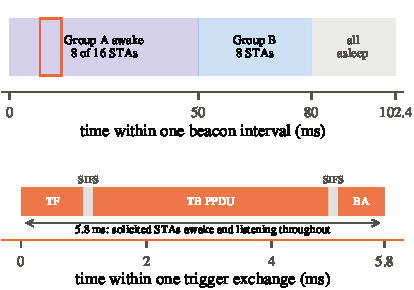
\includegraphics[width=\columnwidth]{figures/fig_system.pdf}
  \caption{\emph{Top:} one beacon interval under a two-group TWT schedule.
  \emph{Bottom:} a trigger exchange on its own scale. A solicited station is
  awake for the whole exchange---receiving, then transmitting its own
  reply---and the scheduler reserves the $5.8$\,ms worst case before admitting
  one, which is what makes uplink OFDMA compete with the schedule.}
  \label{fig:system}
\end{figure}

\subsection{Uplink OFDMA}

When uplink OFDMA is enabled the access point sends a trigger frame naming a
set of stations and the resource unit each may use; those stations reply
simultaneously in a trigger-based PPDU. Contention is replaced by scheduling at
a cost: a solicited station is awake for the whole exchange. This is where the
mechanisms meet---a station outside its service period cannot be solicited, so
OFDMA multiplexes only \emph{within} the awake group while consuming part of
the window the schedule was keeping short. The scheduler solicits at most four
stations per trigger, ns-3's default, against the nine $26$-tone resource units
a $20$\,MHz channel admits; Section~\ref{sec:results} reports both.

\subsection{Control problem}

At decision $t$ the access point observes a state $s_t$ and selects
\begin{equation}
a_t = b_t \cdot 380 + s_t^{\mathrm{sched}} \cdot 19 + g_t,
\label{eq:action}
\end{equation}
with $s^{\mathrm{sched}} \in \{0,\dots,19\}$ a schedule, $g \in \{0,\dots,18\}$
an assignment and $b \in \{0,1\}$ enabling uplink OFDMA for that window: $760$
joint actions. The objective is to minimise station energy without reducing
delivered throughput.

\section{Methodology}
\label{sec:method}

\subsection{State and reward}

The state is a $130$-dimensional vector: two aggregate terms, then eight
features per station. Per station these are throughput, a normalised demand
deficit, three scaled backlog indicators, energy efficiency, drops and energy
drawn. All are deltas over the preceding decision window. The state carries no
clock, so a policy cannot infer the schedule from time alone.

The reward combines a per-station term $r_{\mathrm{sum}}$, Jain fairness
$r_{\mathrm{fair}}$, and a network term $r_{\mathrm{net}}$ containing an energy
penalty. We use
\begin{equation}
r = 0.30\,z\!\left(-\tanh\frac{E}{E^{*}}\right) + 0.55\,z(r_{\mathrm{sum}})
    + 0.15\,z(r_{\mathrm{fair}}),
\label{eq:reward}
\end{equation}
where $E$ is the per-decision energy summed over stations, $E^{*} = 8000$\,mJ,
and $z(\cdot)$ is standardised on the training split alone. The energy scale
matters: the formulation we inherited used $E_0 = 400$\,mJ, which saturates the
$\tanh$ across the whole operating range and leaves the reward insensitive to
energy. Section~\ref{sec:results} quantifies what that correction is worth.

\subsection{Dataset and training}

We log $2{,}404$ episodes, $100{,}235$ transitions (Alg.~\ref{alg:pipeline}).
The ten-decision hold is deliberate: with a fresh draw every decision, measured
energy is flat against schedule tightness, and only a sustained schedule makes
the gradient visible. A uniform behaviour policy is also the conservative
choice. It is the hardest case for offline RL, because the data contains no
competent trajectory to imitate---which is why behaviour cloning finishes last
here---so a deployment logging from a working controller would start from
strictly better coverage of the actions worth taking. Splits are by episode, never by transition---$2{,}043$
training, $361$ held out---and we train behaviour cloning, DQN+CQL, Double DQN,
dueling DQN+CQL and IQL~\cite{kumar2020cql,vanhasselt2016ddqn,kostrikov2022iql}
at ten initialisations each.

\subsection{Checkpoint selection}

Selecting a checkpoint without touching the network is itself a problem.
Importance-sampling estimates are degenerate here: for a deterministic policy
against a behaviour policy uniform over $A$ actions, the effective sample size
reduces to the state-action matches---a few hundred out of $15{,}025$ held-out
transitions. We therefore rank by fitted Q evaluation~\cite{le2019fqe}, fitting
a critic on the training split and evaluating at held-out episode starts, and
validate that ranking against the simulator rather than assume it sound.

\begin{algorithm}[t]
\caption{Offline joint TWT/OFDMA control}
\label{alg:pipeline}
\small
\begin{algorithmic}[1]
\STATE \textbf{Collect} $\mathcal{D}$: for each episode, draw $a \sim \mathrm{Unif}(760)$,
       hold it for $H=10$ decisions, log $(s,a,r,s')$
\STATE \textbf{Split} $\mathcal{D}$ by episode into $\mathcal{D}_{\mathrm{tr}}, \mathcal{D}_{\mathrm{ho}}$
\FOR{each algorithm $m$ and seed $\sigma \in \{42..51\}$}
  \STATE $\theta_{m,\sigma} \leftarrow$ train $m$ on $\mathcal{D}_{\mathrm{tr}}$, snapshot every $50$ epochs
  \STATE $k^\star \leftarrow \arg\max_k \mathrm{FQE}(\theta^{(k)}_{m,\sigma}; \mathcal{D}_{\mathrm{tr}}, \mathcal{D}_{\mathrm{ho}})$
         \COMMENT{no simulator}
\ENDFOR
\STATE \textbf{Deploy} $\theta^{(k^\star)}$: each decision, take
      $a_t = \arg\max_a Q(s_t,a)$, decode $(b_t, s^{\mathrm{sched}}_t, g_t)$,
      and if $b_t$ solicit only stations whose service period has
      $\ge 5.8$\,ms left
\end{algorithmic}
\end{algorithm}

\subsection{Service-period-aligned triggering}

A trigger exchange started near the end of a service period cannot finish inside
it. The station sleeps before it replies, and the access point is left awaiting
a reply from a radio that has switched off. That is a protocol fault, not a
missed transmission opportunity.

We therefore solicit a station only while its service period still has room for
the entire exchange, which we take as $5.8$\,ms, covering the trigger, two short
interframe spaces, a maximum-duration trigger-based PPDU and the acknowledgement.
This aligns uplink OFDMA with the awake window by construction.

\section{Experimental Setup}
\label{sec:setup}

\subsection{Simulator and parameters}

All experiments use ns-3.44 with the ns3-ai interface, which lets a Python
policy act in a running simulation. Table~\ref{tab:config} lists every
parameter, naming the sweep wherever one chose the value.

\begin{table}[t]
\centering
\caption{Simulation and training configuration. Every value is the one used to
produce the reported results; where a sweep chose it, the sweep is named.}
\label{tab:config}
\footnotesize
\setlength{\tabcolsep}{3pt}
\begin{tabular}{lll}
\toprule
\multicolumn{3}{l}{\emph{Scenario} (ns-3.44)} \\
\midrule
stations & $16$ & four device classes, four each \\
channel & $20$\,MHz & 802.11ax, single BSS \\
STAs per trigger & $4$ & ns-3 default; $20$\,MHz fits $9$ \\
CCA-busy current & $273$\,mA & ns-3 default; TX/RX $232/66$ \\
beacon interval & $102.4$\,ms & \\
decision interval $\Delta$ & $20$\,BI $=2.048$\,s & $42$ decisions per episode \\
episode length & $86$\,s & \\
offered load & $0.058/2.037/$ & IoT / camera / voice / \\
 & $0.030/3.400$\,Mb/s & streamer; $22.1$\,Mb/s total \\
load step & $\times\{1.5,2.0,2.5\}$ & in $60\,\%$ of episodes, at \\
 & & $U[30,70]$\,s; seed-determined \\
\midrule
\multicolumn{3}{l}{\emph{Dataset}} \\
\midrule
transitions & $100{,}235$ & $2{,}404$ episodes \\
split & $85{,}210$ / $15{,}025$ & by episode, $2{,}043$ / $361$ \\
behaviour policy & uniform over $760$ & all $760$ actions present \\
\midrule
\multicolumn{3}{l}{\emph{Training} (all five algorithms)} \\
\midrule
network & $130$--$128$--$128$--$760$ & ReLU; dueling splits the head \\
optimiser & Adam, lr $10^{-3}$ & defaults otherwise \\
batch size & $512$ & $149$ steps per epoch \\
epochs & $200$ & milestone every $50$ \\
discount $\gamma$ & $0.95$ & \\
Bellman target clip & $\pm 50$ & chosen so $|V| = 23$--$35$ fits \\
CQL coefficient $\alpha$ & $0.5$ & from an FQE sweep over \\
 & & $\{0.5, 1.0, 2.0\}$ \\
IQL expectile & $0.7$ & \\
training seeds & $42$--$51$ & ten independent fits per \\
 & & algorithm (Table~\ref{tab:main}) \\
\midrule
\multicolumn{3}{l}{\emph{Selection and evaluation}} \\
\midrule
model selection & FQE, $3\times10^4$ iters & episode-disjoint holdout \\
convergence gate & none & see Section~\ref{sec:results} \\
evaluation seeds & $50$ shared & disjoint from training \\
heuristic tuning seeds & $15$ & $80000$--$80014$, disjoint \\
\bottomrule
\end{tabular}
\end{table}


\subsection{Seeds and protocol}

Three disjoint seed sets are used, so no policy is evaluated on data that
informed it: collection from $30000$, tuning on $80000$--$80014$, and all
reported results on $90000$--$90049$.

The fifty evaluation seeds are \emph{paired}: a seed fixes the traffic, the time
of any load change and its multiplier, so every policy meets an identical
environment. Pairing removes environment variance, which is what lets fifty
seeds resolve differences that would otherwise need many more. Energy is
reported over the $42$-decision control window, excluding the warm-up.

\subsection{Baselines}

Nine non-learned scenarios span the configuration space, from no power save to a
tuned hand-designed controller; Table~\ref{tab:main} lists them.

That controller is the comparator that matters: a delay-triggered hysteresis
rule raising the duty cycle when observed delay crosses an upper threshold and
lowering it below a lower one. Its thresholds, schedule pair and OFDMA mode come
from a staged coordinate search on the tuning seeds, minimising energy subject
to a service floor, so it cannot win by refusing traffic. The static baseline is
chosen the same way.

\section{Results}
\label{sec:results}

\begin{table*}[t]
\centering
\caption{Every scenario on the same $50$ paired evaluation seeds, one
simulator and one $42$-decision measurement window. Where uplink OFDMA is
enabled the scheduler is service-period aligned and the sleep guard is
disabled, so no row depends on that workaround. The hand-designed controller
is tuned on disjoint seeds under a service floor; the row marked
\emph{free choice} lets that search pick its own OFDMA mode, and it picks
off. Learned rows give the mean and standard deviation over $10$ training
seeds. The last three columns compare each learned method against the
\emph{free choice} controller at $166.5$\,J, Wilcoxon signed-rank:
\emph{mean over runs} averages the ten fits per seed; \emph{oracle}
is each method's lowest-energy fit, selected on the same evaluation seeds
it is scored on, and is therefore retrospective. \emph{backlog} is a
drain-time proxy, per-station queue bytes over that station's offered
rate, averaged over stations and decisions; it is not a measured packet
latency. $>$3\,s is the fraction of decisions whose mean proxy exceeds
three seconds. OFDMA: share of decisions with the scheduler enabled.}
\label{tab:main}
\footnotesize
\setlength{\tabcolsep}{4.5pt}
\begin{tabular}{lrrrrrrrr}
\toprule
 & & & & & & \multicolumn{2}{c}{mean over runs} & oracle \\
\cmidrule(lr){7-8}\cmidrule(lr){9-9}
Scenario & $E$ (J) & tput (Mb/s) & backlog (ms) & $>$3\,s & OFDMA & $\Delta$ vs hand & $p$ & $\Delta$ vs hand \\
\midrule
No TWT, no OFDMA & $441.1$ & $24.95$ & $2637$ & $0.24$ & $0\,\%$ & & & \\
Static TWT & $173.3$ & $21.03$ & $2789$ & $0.37$ & $0\,\%$ & & & \\
Static TWT $+$ OFDMA & $282.2$ & $19.82$ & $2823$ & $0.40$ & $100\,\%$ & & & \\
Random TWT & $171.1$ & $14.47$ & $3159$ & $0.63$ & $0\,\%$ & & & \\
Random TWT $+$ OFDMA & $228.5$ & $13.51$ & $3188$ & $0.66$ & $100\,\%$ & & & \\
OFDMA only, no TWT & $477.8$ & $24.30$ & $2652$ & $0.25$ & $100\,\%$ & & & \\
Random joint action & $198.8$ & $14.29$ & $3157$ & $0.63$ & $48\,\%$ & & & \\
Hand-designed, OFDMA on & $265.5$ & $18.37$ & $2904$ & $0.43$ & $100\,\%$ & & & \\
Hand-designed, \emph{free choice} & $166.5$ & $19.22$ & $2888$ & $0.41$ & $0\,\%$ & & & \\
\midrule
\multicolumn{9}{l}{\emph{offline RL, 10 training seeds each}} \\
\quad IQL & $107.3 \pm 2.6$ & $20.76$ & $2805$ & $0.38$ & $0\,\%$ & $-35.6\,\%$ & $10^{-15}$ & $-37.2\,\%$ \\
\quad DQN$+$CQL & $193.0 \pm 10.1$ & $20.54$ & $2829$ & $0.40$ & $23\,\%$ & $+15.9\,\%$ & $10^{-5}$ & $+1.6\,\%$ \\
\quad Dueling$+$CQL & $194.1 \pm 14.7$ & $20.49$ & $2834$ & $0.40$ & $25\,\%$ & $+16.6\,\%$ & $10^{-6}$ & $+0.7\,\%$ \\
\quad DDQN & $222.7 \pm 13.5$ & $15.64$ & $3076$ & $0.58$ & $43\,\%$ & $+33.8\,\%$ & $10^{-15}$ & $+23.7\,\%$ \\
\quad BC & $255.1 \pm 12.4$ & $19.78$ & $2875$ & $0.43$ & $48\,\%$ & $+53.2\,\%$ & $10^{-15}$ & $+42.7\,\%$ \\
\bottomrule
\end{tabular}
\end{table*}


\subsection{The two mechanisms do not combine}

Table~\ref{tab:main} holds three pairs differing only in the OFDMA bit, and in
each enabling it costs energy: $+62.8\,\%$ under the static schedule,
$+33.6\,\%$ under random TWT, $+8.3\,\%$ with TWT off.

Throughput falls in all three, so this is not a throughput-for-energy trade.

The ordering is the informative part: the penalty is largest where TWT sleeps
hardest and smallest where it does not sleep at all, because soliciting a
station competes with the schedule trying to keep it asleep.

\subsection{The cost is carrier sensing, not lost sleep}

Our first explanation was that triggers wake sleeping stations. The traces
refute it. Mean sleep occupancy---the fraction of the control window a station
spends in PHY sleep, averaged over the sixteen---differs by under $0.8$
percentage points between the OFDMA arms. Stations sleep just as much; their
awake time simply costs more.

Per-state traces from a separate instrumented run---the tuned controller with
and without the scheduler, which differ by $113.7$\,J there---place $69\,\%$
of the extra energy in carrier-sense busy and $24\,\%$ in receive, $9\,\%$ in
transmit, against $-1\,\%$ in idle. A solicited station is awake across the
trigger, its own transmission and the acknowledgement, and the awake portion
outside its own transmission is charged at the CCA-busy current.

The scenario leaves CCA-busy at ns-3's default $273$\,mA against its own
$66$\,mA receive current---an internally inconsistent parameterisation---so we
re-evaluated every load-bearing arm at $66$\,mA, same policies and seeds.
Energies fall $21$--$27\,\%$ unevenly, but both conclusions hold: OFDMA costs
$+57.8\,\%$ rather than $+62.8\,\%$ under the static schedule, and IQL beats
the controller by $31.2\,\%$ ($84.6$ against $123.1$\,J) rather than
$35.6\,\%$. Signs survive the power profile; magnitudes do not.

\subsection{One algorithm beats the tuned rule}

Given a free choice the tuned controller disables OFDMA, worth $99$\,J
($265.5$ against $166.5$\,J); we take that stronger form as the baseline.


IQL reaches $107.3 \pm 2.6$\,J, the spread being the standard deviation over
ten training runs, not a confidence interval. That is a $35.6\,\%$ reduction;
the interval $[-36.5,-34.7]\,\%$ is a paired bootstrap over the fifty shared
seeds of the per-seed mean across runs, and $p = 1.8\times10^{-15}$ is a
two-sided Wilcoxon signed-rank test on the same pairing. Neither propagates
uncertainty from resampling training runs; the across-run spread is reported
separately. The reduction comes with higher
mean throughput, $20.76$ against $19.22$\,Mb/s, and a backlog proxy lower by
$83$\,ms ($p = 9.8\times10^{-9}$ paired); the change in the fraction of
decisions above three seconds is not statistically detectable ($p = 0.07$). Its worst fit of ten,
$112.4$\,J, still beats every other method's best.

That column is a drain-time proxy---queue bytes over offered rate---not a
measured latency, so it tracks standing backlog: flat across all $42$ decisions,
$2.6$--$2.9$\,s where throughput stays near offered load and $3.1$--$3.2$\,s
where it does not. We use it as a guard against starving traffic, not as a
latency claim.

\subsection{Four of five do not, and selection is why}

Table~\ref{tab:main} is why we claim this for IQL and not for offline RL as a
family. The \emph{mean over runs} column averages the ten fits per evaluation
seed, estimating expected performance over training randomness: DQN$+$CQL is
$15.9\,\%$ worse than the hand-designed rule ($p = 8.6\times10^{-5}$),
dueling DQN$+$CQL $16.6\,\%$ worse ($p = 4.3\times10^{-6}$), DDQN and
behaviour cloning worse still.

The \emph{oracle} column takes each method's lowest-energy fit, chosen on the
same seeds it is then scored on. There the CQL variants sit within $1.6\,\%$ of
the baseline with no difference detected ($p = 0.74$, $0.55$)---a failure to
detect, not evidence of equivalence, under retrospective selection. The gap
between the columns is what matters: expected performance over training
randomness is $16\,\%$ worse than a hand-written rule, while a retrospectively
chosen fit is not distinguishable from it. Whether an off-policy estimator can
pick that fit in advance across independent runs is open; we validate FQE only
for ranking checkpoints within a run.

IQL is the exception because it barely varies: its across-fit standard deviation
is $2.6$\,J against $10.1$ to $14.7$\,J for the others, so which fit you deploy
does not matter.

\begin{figure}[t]
  \centering
  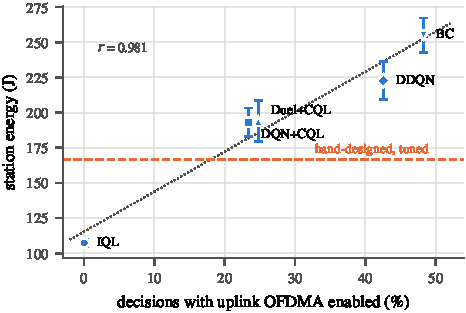
\includegraphics[width=\columnwidth]{figures/fig_ordering.pdf}
  \caption{Station energy against how often each learned policy enables uplink
  OFDMA; bars are the standard deviation over ten training runs. The association
  across these five algorithm-level means is strong ($r = 0.981$, $n=5$) but
  descriptive: the methods differ in schedule and grouping too. Dashed: the
  tuned controller.}
  \label{fig:ordering}
\end{figure}

\subsection{What separates the methods is the OFDMA bit}

The five methods order by energy as they order by how often they enable the
scheduler (Fig.~\ref{fig:ordering}), from IQL at $0\,\%$ to behaviour cloning
at $48\,\%$---the last because the logger chose the bit by coin flip and
imitating it reproduces that.

The lowest-energy method is the one that disables the scheduler, and the
coordinate search reaches the same configuration independently. The obvious objection is that we crippled the scheduler: ns-3 solicits four
stations per trigger by default, while schedule~11 leaves eight awake and the
channel admits nine resource units, so half the awake set was unreachable.
Raising the limit to nine makes uplink OFDMA worse, not better---$+87.4\,\%$
against the no-OFDMA arm instead of $+62.8\,\%$ under the static schedule, and
$+83.3\,\%$ instead of $+59.5\,\%$ for the hand-designed controller, both
$+15\,\%$ on the default at $p = 2\times10^{-15}$ with throughput falling at
each step. Solicitation cost scales with the stations a trigger names; the
benefit scales with the data they have, and in this mix they have little.

Each seed either holds its offered load constant or steps it by $1.5$ to
$2.5\times$ partway through. Splitting the fifty on that flag gives $35.1\,\%$
below the baseline on the $19$ constant-load seeds ($p = 3.8\times10^{-6}$) and
$35.8\,\%$ on the $31$ stepped ones ($p = 9.3\times10^{-10}$): robustness to
within-distribution load variation, not transfer to unseen traffic.

\subsection{Is the adaptation necessary?}

IQL and the tuned controller both disable uplink OFDMA, so the gap between them
cannot come from that bit. Would one well-chosen fixed configuration do as
well? We swept all $20$ schedules at the deployed grouping on the tuning seeds
with OFDMA off, picked the Pareto-efficient ones from tuning data alone, and
evaluated those on the untouched evaluation seeds.

None matches IQL. At its energy the best fixed schedule delivers
$12.62$\,Mb/s against $20.76$---$64\,\%$ more data for the same power, with the
energy difference undetectable ($p = 0.12$); at its throughput the best fixed
schedule costs $179.1$\,J against $107.3$, so IQL is $40\,\%$ cheaper. One
schedule is beaten on both axes at once ($145.4$\,J, $17.93$\,Mb/s), and on the
tuning seeds no schedule of the twenty comes within $10\,\%$ of IQL's energy at
$90\,\%$ of its throughput.

The traces say why. IQL uses $14.9$ distinct actions per $42$-decision
episode, and the schedules it favours are poor alone: schedule~18 for
$43\,\%$ of decisions and schedule~19 for $23\,\%$ deliver $15.64$ and
$12.74$\,Mb/s as fixed policies. Holding either costs about what IQL costs
while moving a third less data, so the gain is in moving between schedules, not
in any one. We swept schedules at the deployed grouping only, so this is the
best fixed \emph{schedule}, not the best of all $380$ configurations.

\subsection{Validation}

Four instrumentation faults materially affected earlier evaluations, each
invisible in aggregate statistics: a convergence gate that discarded a sound
checkpoint ranking ($6.5\,\%$ energy); a saturated reward energy term
($13.3$\,J, though the unrepaired reward still beat the baseline by
$27.5\,\%$); two harnesses whose measurement windows differ by a warm-up; and
an $8$\,ms sleep deferral applied only with the OFDMA bit set, worth
$+62.0\,\%$ alone---two thirds of a penalty we had charged to the protocol,
and one that moved sleep \emph{occupancy} under $0.8\,\%$.

\section{Conclusion}
\label{sec:conclusion}

A controller for TWT and uplink OFDMA has to adapt, and neither obvious way of
obtaining one is satisfactory: a hand-coded rule needs an expert and is tuned
for conditions that change, while an online learner has to explore on a network
carrying real users. We tested the middle path. Five offline algorithms were
trained on $100{,}235$ logged transitions in ns-3.44, ten initialisations each,
selecting a TWT schedule, a group assignment and the uplink OFDMA bit per
decision window---$760$ actions---and compared against nine non-learned
scenarios on fifty paired seeds under one simulator and one window.

Two findings follow. First, IQL reduces station energy by $35.6\,\%$ against a
hand-designed controller tuned under a service floor, at higher throughput and
consistently across ten fits. Second, the two mechanisms substitute rather than
combine here: enabling uplink OFDMA raises energy at every TWT setting tested,
the five methods order by how often each enables it, and an independent
coordinate search disables it when given the choice.

The result is about IQL, not offline RL. Four of five methods lose to the
hand-designed rule, and the two CQL variants tie only if their best of ten fits
can be identified---which takes the network measurements the method was adopted
to avoid. Low across-fit variance is what makes IQL usable, so checkpoint
selection, not policy optimisation, is the remaining difficulty.

Three limits bound the claims. The topology is one basic service set, sixteen
stations and $20$\,MHz; we tested solicitation limits of four and nine and the
substitution strengthened at both, but we cannot speak beyond them. The station
mix and the traffic model are identical across every arm, so the comparisons are
internally controlled but not shown to transfer. The energy model also mixes two power profiles, leaving CCA-busy at ns-3's
default $273$\,mA---measured on an 802.11n laptop
card~\cite{halperin2010demystifying}---against its own $66$\,mA receive
current. Re-evaluating at $66$\,mA moves arm energies by $21$ to $27\,\%$ and
unevenly, yet changes no ordering and neither conclusion
(Section~\ref{sec:results}); since the policies were trained under the shipped
profile, that repricing measures the same behaviour under a different energy
model, not what a policy would have learned under it. Finally the logged actions were held for ten decisions; deploying at that
cadence changes energy by $-1.0\,\%$ ($p = 0.12$), so the mismatch does not
appear to bite.

Whether the substitution reverses at the higher station counts, wider channels
and larger solicitation sets where uplink OFDMA is expected to pay is the
natural next step.




\bibliographystyle{IEEEtran}
\bibliography{refs}

\end{document}
